\section{Dominancia operátorok}\label{sec:DOMINANCIA_OPERATOROK}
A multikritériumú genetikus algoritmusok esetén felmerül a kérdés, hogy miként döntjük el, hogy egy megoldás jobb-e vagy rosszabb, mint egy másik.
Viszont az is megtörténhet, hogy két megoldás összehasonlíthatatlan.
Ennek a kérdésnek a megválaszolása érdekében szükséges bevezetnünk a \emph{dominancia operátor} fogalmát.
A dominancia operátor fontos szerepet lát el a multikritériumú genetikus algoritmusok keretein belül,
mivel a \emph{dominancia reláció} segítségével lesz eldöntve, hogy két megoldás közül melyik dominálja melyiket, vagy hogy egyik sem dominálja a másikat.
Az NSGAII multikritériumú genetikus algoritmus esetén több típusú dominanciát fogunk kipróbálni kísérleti célokból.
Ezeket a dominancia típusokat szeretnénk a következőkben ismertetni.


\subsection{Pareto-dominancia}
\begin{ert}
  Azt mondjuk, hogy egy $x$ megoldás \emph{Pareto-dominál} egy $y$ megoldást $\left( x \prec y \right)$, ha teljesül a következő két feltétel:
  \begin{align*}
    \forall i \in \left\{ 1, 2, \dots, \abs{F} \right\} \colon f_i(x) \leq f_i(y), \\
    \exists j \in \left\{ 1, 2, \dots, \abs{F} \right\} \colon f_j(x) < f_j(y).
  \end{align*}
\end{ert}

Tehát az $x$ megoldás minden szempontból legalább olyan jó, mint az $y$, és legalább egy szempontból még jobb is nála.


% \subsubsection{Pareto-optimum}
\begin{ert}
  A Pareto-dominancia segítségével bevezethetjük az optimum fogalmát.
  Egy $\hat{x}$ \emph{Pareto-optimum}, ha nincs még egy olyan megoldásjelölt, ami dominálná őt:
  \[
    \nexists x \in \mathbb{P} \colon x \prec \hat{x}.
  \]
\end{ert}


% \subsubsection{Pareto-front}
\begin{ert}
  Gyakran megtörténik, hogy nem csak egy, hanem több Pareto-optimális megoldásunk van.
  Ebben az esetben a Pareto-optimális megoldások halmazát nevezzük \emph{Pareto-frontnak}.
\end{ert}


% \subsubsection{Egy példa}
\begin{pld}
  \Aref{fig:PARETO_DOMINANCE}. ábra egy példát mutat a Pareto-optimumokra.
  A probléma két célfüggvény optimalizálásából tevődik össze: az $f_1$ célfüggvény maximalizálásából és az $f_2$ célfüggvény minimalizálásából.
  Tehát egy pont minél távolabb van az origótól az X-tengelyen, de ugyanakkor minél közelebb hozzá az Y-tengelyen, annál jobb.

  Néhány következtetés, ami leolvasható a diagramról:
  \begin{itemize}
    \item[\textbullet] $A \prec B$, mivel mindkét szempont szerint jobb nála;
    \item[\textbullet] $E \prec A$, mivel $f_2$ szempontjából azonosak, de $f_1$ szerint jobb;
    \item[\textbullet] $A \nprec D$, mert bár $f_2$ szerint jobb, de $f_1$ szempontjából rosszabb;
    \item[\textbullet] $D \nprec A$, mert bár $f_1$ szerint jobb, de $f_2$ szempontjából rosszabb;
    \item[\textbullet] $C$, $E$ pontokat senki se dominálja (ők se egymást), ezért ők alkotják a Pareto-frontot.
  \end{itemize}

  Jól látható, hogy a feladatnak nincs egyértelmű megoldása.
  A $C$ és $E$ pontok nem azonosak, mégsem tudjuk az egyiket előnyben részesíteni a másikhoz képest.
  A feladat megoldása tehát ez a két pont.
\end{pld}

\begin{meg}
  Fontos megemlítenünk, hogy ez nem hátrány, hanem éppenhogy előny.
  A Pareto-dominancia lehetővé teszi, hogy ne csak egy megoldást kapjunk vissza, hanem akár mindet.
  A többcélú feladatok megoldásánál éppen azt szeretnénk, hogy minél több nem-dominált eredményt kapjunk.
  Mivel legtöbbször a front mérete nagyon nagy, és az összes megoldást nem várhatjuk el, akkor az egymástól minél távolibbakat szeretnénk megkapni.

  Az, hogy utána melyik megoldás lesz kiválasztva, az már a felhasználó egyéni döntése.
\end{meg}

\begin{figure}[t]
  \centering
  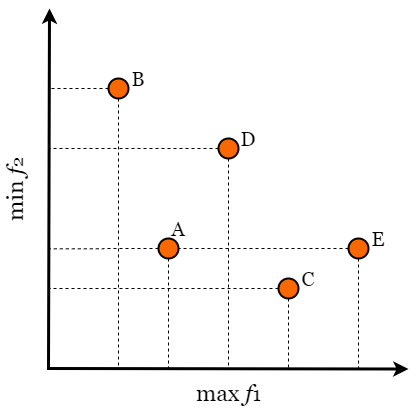
\includegraphics[scale=0.5]{images/pareto_dominance.png}
  \caption{
    Példa egy kétcélú optimalizálási feladatra, ahol az $f_1$ célfüggvényt maximalizálni, míg az $f_2$ célfüggvényt minimalizálni kell.
  }
  \label{fig:PARETO_DOMINANCE}
\end{figure}


\subsection{Nash-dominancia}\label{subsec:NASH_DOMINANCIA}
A Nash-dominancia fogalmát \citeN{lung2008computing} vezették be, és a Nash-egyensúly fogalmán alapszik.
Megértéséhez szükséges néhány, a \emph{játékelméletből} \cite{von2007theory} ismert fogalom bevezetése.


\subsubsection{Nem-kooperatív játékok}
Legyen $n > 1$ természetes szám a játékosok száma, és $I = \left\{ 1, \dots, n \right\}$ a játékosok halmaza.
Minden $i \in I$ esetén, $S_i$ az $i$-edik játékos stratégiáinak a halmaza, míg $s_i \in S_i$ a játékos tetszőleges stratégiája.
Legyen $S = S_1 \times S_2 \times \dotsc \times S_n$ a stratégiaprofilok halmaza, $s \in S$ pedig egy általános stratégiaprofil.
Minden $i \in I$ esetén, $u_i \colon S \to \mathbb{R}$ az $i$-edik játékos kifizetőfüggvénye.
Legyen $U = \left\{ u_1, \dots, u_n \right\}$ a kifizetőfüggvények halmaza.
Jelölje $\left( s_i, s^*_{-i} \right)$ az $\left( s^*_1, \dots, s^*_{i-1}, s_i, s^*_{i+1}, \dots, s^*_n \right)$ stratégiaprofilt,
amelyet úgy kapunk, hogy az $s^*$ stratégiaprofil $i$-edik játékosának a stratégiáját kicseréljük $s_i$-re, $s_i \in S_i$.


\subsubsection{Nash-egyensúly}
Az előbb bevezetett jelölések segítségével bevezethetjük a nem-kooperatív játékelmélet központi fogalmát, a \emph{Nash-egyensúlyt} \cite{nash1951non}.

\begin{ert}
  Azt mondjuk, hogy az $s^* \in S$ stratégiaprofil Nash-egyensúlyt alkot,
  ha egyik játékosnak sem érdemes egyoldalúan eltérnie a stratégiaprofilban szereplő saját stratégiájától.
  Tehát minden $i \in I$ játékos és $s_i \in S_i$ stratégia esetén, a következő egyenlőtlenség teljesül:
  \[
    u_i\left(s^*\right) \ge u_i\left(s_i, s_{-i}^*\right).
  \]
\end{ert}


\subsubsection{Nash-dominancia}\label{subsubsec:NASH_DOMINANCIA}
Legyen $x$ és $y$ két stratégiaprofil $S$-ből.
Bevezetünk egy $k \colon S \times S \to \mathbb{N}$ operátort, amely az $\left( x, y \right)$ pároshoz hozzárendeli a következő halmaz számosságát:
\[
  \left\{ i \in I \mid u_i(y_i, x_i) \ge u_i(x), y_i \neq x_i \right\}.
\]

A halmaz azon $i$ játékosokat tartalmazza, akik adott $x$ stratégiaprofil esetén, hasznot húznának abból, ha megváltoztatnák stratégiájukat $x_i$-ről $y_i$-re.

\begin{ert}
  Azt mondjuk, hogy egy $x$ stratégiaprofil \emph{Nash-dominál} egy $y$ stratégiaprofilt ($x \prec y$), ha teljesül az alábbi feltétel:
  \begin{equation}\label{eqn:NASH_DOMINANCIA}
    k(x,y) < k(y, x).
  \end{equation}
\end{ert}

Tehát egy $x$ stratégiaprofil akkor Nash-dominál egy $y$ stratégiaprofilt, ha kevesebb játékos tudja megnövelni nyereségét úgy, hogy megváltoztatja stratégiáját $x_i$-ről $y_i$-re, mint fordítva.
Azt is mondhatjuk, hogy az $x$ stratégiaprofil stabilabb (közelebb van az egyensúlyhoz), mint az $y$ stratégiaprofil.


% \subsubsection{Nash-optimum}
A Nash-dominancia segítségével bevezethetjük az optimum fogalmát.

\begin{ert}
  Egy $s^* \in S$ stratégiaprofil \emph{Nash-optimum}, ha nincs még egy olyan stratégiaprofil, ami dominálná őt:
  \[
    \nexists s \in S, s \neq s^* \colon s \prec s^*.
  \]
\end{ert}


% \subsubsection{Nash-front}
\begin{ert}
  Gyakran megtörténik, hogy nem csak egy, hanem több Nash-optimális megoldásunk van.
  Ebben az esetben a Nash-optimális megoldások halmazát nevezzük \emph{Nash-frontnak}.
\end{ert}


% \subsubsection{Nash és a BOCNDP}
\begin{tet}\label{thm:PROFIL_NE_DOMINANCIAVAL}
  \citeN{lung2008computing} bebizonyították, hogy egy $s^* \in S$ stratégiaprofil akkor és csakis akkor Nash-egyensúly, ha
  \[
    \forall s \in S \colon k(s^*, s) = 0
  \]
  teljesül.
\end{tet}

\begin{tet}\label{thm:NE_EGYENLO_NF}
  \citeN{lung2008computing} egy fontos következtetésre jutottak, miszerint minden Nash-egyensúlyt alkotó stratégiaprofil egyben Nash-optimum is, és minden Nash-optimum egyben Nash-egyensúlyt alkotó stratégiaprofil is.
\end{tet}

\begin{meg}
  \Aref{thm:PROFIL_NE_DOMINANCIAVAL}. és \aref{thm:NE_EGYENLO_NF}. tételek azért rendkívül fontos eredmények, mivel lehetővé teszik számunkra, hogy evolúciós kereső operátorok (keresztezés, mutáció, kiválasztás) segítségével megkeressük a Nash-egyensúlyt alkotó megoldásokat.
\end{meg}


% \subsubsection{Egy példa}
A következőkben egy példán keresztül szeretnénk szemléltetni a Nash-dominancia és a Nash-egyensúly közötti kapcsolatot.

\begin{figure}[t]
  \begin{minipage}{\textwidth}
    \begin{minipage}[b]{0.3\textwidth}
      \centering
      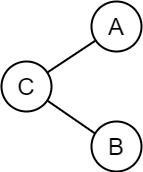
\includegraphics[scale=0.5]{images/nash_dominance.png}
      \vspace*{2.5mm}
      \captionof{figure}{Példa egy három csomópontból álló útgráfra.}
      \label{fig:NASH_DOMINANCE}
    \end{minipage}
    \hfill
    \begin{minipage}[b]{0.65\textwidth}
      \centering
      \resizebox{0.8\textwidth}{!}{
        \begin{tabular}{ccccc}
                                                             &                                 & \multicolumn{2}{c}{Második játékos} &                                                                   \\ \cline{2-5}
          \multicolumn{1}{c|}{}                              & \multicolumn{1}{c|}{}           & \multicolumn{1}{c|}{\textit{A}}     & \multicolumn{1}{c|}{\textit{B}} & \multicolumn{1}{c|}{\textit{C}} \\ \cline{2-5}
          \multicolumn{1}{c|}{\multirow{2}{*}{Első játékos}} & \multicolumn{1}{c|}{\textit{A}} & \multicolumn{1}{c|}{$1; 1$}         & \multicolumn{1}{c|}{$1; 1$}     & \multicolumn{1}{c|}{$1; 0$}     \\ \cline{2-5}
          \multicolumn{1}{c|}{}                              & \multicolumn{1}{c|}{\textit{B}} & \multicolumn{1}{c|}{$1; 1$}         & \multicolumn{1}{c|}{$1; 1$}     & \multicolumn{1}{c|}{$1; 0$}     \\ \cline{2-5}
          \multicolumn{1}{c|}{}                              & \multicolumn{1}{c|}{\textit{C}} & \multicolumn{1}{c|}{$0; 1$}         & \multicolumn{1}{c|}{$0; 1$}     & \multicolumn{1}{c|}{$0; 0$}     \\ \cline{2-5}
        \end{tabular}
      }
      \captionof{table}{A bal oldalon található gráf leképezése egy kétszemélyes stratégiai játékra.}
      \label{tab:NASH_DOMINANCE}
    \end{minipage}
  \end{minipage}
\end{figure}

\begin{pld}\label{pld:NASH_DOMINANCE}
  \Aref{fig:NASH_DOMINANCE}. ábrán látható gráfban $k = 1$ kritikus csomópontot szeretnénk beazonosítani.
  \Aref{eqn:PAIRWISE_CONNECTIVITY} képlettel leírt célfüggvény minimalizálása. leírt függvényt fogjuk használni, mint célfüggvény vagy kifizetőfüggvény.
  Ez fogja megmondani, hogy egy megoldás vagy stratégiaprofil mennyire jó.
  Célunk a függvény minimalizálása \ref{eqn:MIN_PAIRWISE_CONNECTIVITY}, mivel minél kisebb értéket ad vissza, annál jobb az illető megoldás.

  A feladatot felfoghatjuk ugyanakkor, mint egy kétszemélyes stratégiai játék.
  \Aref{tab:NASH_DOMINANCE}. táblázat szemlélteti a feladat lemodellezett változatát, mint kétszemélyes stratégia játék:
  $I = \left\{ 1, 2 \right\}$ a játékosok halmaza, $S_1 = S_2 = \left\{ A, B, C \right\}$ a stratégiahalmazok, a kifizetéseket a mátrix tartalmazza.

  A Nash-egyensúly megtalálása érdekében mindegyik stratégiaprofilt sorra meg kell vizsgáljuk.
  Ne felejtsük, hogy célunk a kifizetőfüggvények minimalizálása.

  \begin{itemize}
    \item[$(A, A)$] -- A $C$ stratégiát választva az $A$ helyett, az első játékos előnyhöz jut, hiszen $u_1(C, A) = 0 < 1 = u_1(A, A)$.
          Ezért ez a stratégiaprofil nem alkot Nash-egyensúlyt.
          Továbbá a második játékos is megnövelheti nyereségét, ha $A$ helyett $C$-t választ, mivel $u_2(A, C) = 0 < 1 = u_2(A, A)$.
    \item[$(A, B)$] -- Ugyanaz a helyzet, mint az $(A, A)$ stratégiaprofil esetén, ezért nem alkot Nash-egyensúlyt.
    \item[$(A, C)$] -- A $C$ stratégiát választva az $A$ helyett, az első játékos előnyhöz jut, hiszen $u_1(C, A) = 0 < 1 = u_1(A, A)$.
          Ezért ez a stratégiaprofil nem alkot Nash-egyensúlyt.
    \item[$(B, A)$] -- Ugyanaz a helyzet, mint az $(A, A)$ stratégiaprofil esetén, ezért nem alkot Nash-egyensúlyt.
    \item[$(B, B)$] -- Ugyanaz a helyzet, mint az $(A, A)$ stratégiaprofil esetén, ezért nem alkot Nash-egyensúlyt.
    \item[$(B, C)$] -- Ugyanaz a helyzet, mint az $(A, C)$ stratégiaprofil esetén, ezért nem alkot Nash-egyensúlyt.
    \item[$(C, A)$] -- A $C$ stratégiát választva az $A$ helyett, a második játékos előnyhöz jut, hiszen $u_2(C, C) = 0 < 1 = u_2(C, A)$.
          Ezért ez a stratégiaprofil nem alkot Nash-egyensúlyt.
    \item[$(C, B)$] -- Ugyanaz a helyzet, mint a $(C, A)$ stratégiaprofil esetén, ezért nem alkot Nash-egyensúlyt.
    \item[$(C, C)$] -- Egyik játékos sem tudja megnövelni nyereségét úgy, hogy a jelenlegi stratégiája helyett egy másikat választ.
          Ezért ez a stratégiaprofil Nash-egyensúlyt alkot.
  \end{itemize}

  Következtetésként elmondhatjuk, hogy ennek a játéknak egy Nash-egyensúlya van, ami nem más, mint a $(C, C)$ stratégiaprofil.

  Ha \aref{sec:KISERLETI_ELOKESZITES}. részben bemutatott NSGAII multikritériumú genetikus algoritmus esetén lecseréljük az általa használt Pareto-dominanciát Nash-dominanciára,
  akkor az algoritmus által meghatározott Nash-front egyetlen Nash-optimális megoldásból fog állni, ami nem lesz más, mint az $S = \left\{ C \right\}$ megoldáshalmaz.

  Láthatjuk, hogy \aref{thm:NE_EGYENLO_NF}. tétel igaz, vagyis használhatjuk a multikritériumú genetikus algoritmusokat Nash-egyensúly egyensúlypont-keresésre.
\end{pld}


\subsection{Berge-dominancia}
A Berge-dominancia fogalmát \citeN{gasko2014characterization} vezették be, és a Berge-egyensúly fogalmán alapszik.
Ugyanúgy, mint \aref{subsec:NASH_DOMINANCIA}. részben bemutatott Nash-dominancia esetén, a Berge-dominancia fogalmának megértéséhez is szükséges először a Berge-egyensúly fogalmát bevezetnünk.


\subsubsection{Berge-egyensúly}
A \emph{Berge-egyensúly} fogalmát \citeN{berge1957theorie} vezette be, de mivel nem látta el konkrét definícióval, ezért jelen formájában \citeN{zhukovskii1994linear} definiálták először.
Nagyon hasonló a közismert Nash-egyensúlyhoz, viszont itt az altruizmus egy formája jelenik meg a nem-kooperatív játék helyett.
A Berge-egyensúly esetén egy stratégiai játék minden játékosa arra törekszik, hogy a többi játékos nyereségét maximalizálja, míg Nash-egyensúly esetén minden játékos a saját kifizetését igyekszik maximalizálni.

\begin{ert}
  Azt mondjuk, hogy az $s^*$ stratégiaprofil Berge-egyensúlyt alkot, ha
  \[
    u_i(s^*) \ge u_i(s^*_i, s_{-i})
  \]
  minden $i \in I$ játékos és $s_{-i} \in S_{-i}$ stratégia esetén teljesül.
\end{ert}

Tehát minden játékos a saját kifizetését próbálja maximalizálni ugyanúgy, mint a Nash-egyensúly esetében.
A különbség azonban onnan adódik, hogy a játékosok nem azt nézik meg, hogy a lehetséges stratégiáik közül melyik az, amelyik a legnagyobb nyereséget hozza számukra,
hanem azt, hogy a többi játékos, ha a jelenlegi stratégiájától egy különböző stratégiát játszik ki, akkor ez megnöveli-e a bevételüket.

A fentieket úgy is megfogalmazhatjuk, hogy nem azt kérdezzük a játékosoktól, hogy milyen akciót választanak, hanem azt, hogy milyen $s_{-i}$ esetén hajlandók beleegyezni, hogy ők $s^*_i$-t válasszanak.
Vagyis a kérdés nem arra vonatkozik, hogy az $i$-edik játékos milyen stratégiát választ, hanem arra, hogy milyen feltételek mellett hajlandó belemenni abba, hogy egy meghatározott stratégiát játsszon.

Berge-egyensúly esetén egyik játékos sem szeretne a többi játékos stratégiáján változtatni.


% \subsubsection{Egy példa}
A következőkben egy példán keresztül szeretnénk szemléltetni a Berge-egyensúly és a Nash-egyensúly közötti különbségeket.

\begin{pld}
  \Aref{tab:BERGE_EGYENSULY}. táblázattal szemléltetett játékban $I = \left\{1, 2\right\}$ a játékosok és $S_1 = S_2 = \left\{A, B\right\}$ a játékosok stratégiáinak a halmaza.

  A Berge-egyensúly megtalálása érdekében mindegyik stratégiaprofilt sorra meg kell vizsgáljuk.
  A Nash-egyensúlynál megadott példával ellentétben (lásd \aref{pld:NASH_DOMINANCE}. példát) itt a kifizetőfüggvények maximalizálása a célunk.

  \begin{itemize}
    \item[$(B, B)$] -- Az első játékos szemszögéből, ha a második játékos megváltoztatja stratégiáját $B$-ről $A$-ra, akkor előnyhöz jut, hiszen $u_1(B, A) = 25 > 10 = u_1(B, B)$.
          Ezért ez a stratégiaprofil nem alkot Berge-egyensúlyt.
          Továbbá a második játékos szemszögéből, ha az első játékos változtatná meg stratégiáját $B$-ről $A$-ra, akkor megnövelhetné nyereséget, mivel $u_2(A, B) = 25 > 10 = u_2(B, B)$.
    \item[$(A, B)$] -- Az első játékos szemszögéből, ha a második játékos megváltoztatja stratégiáját $B$-ről $A$-ra, akkor előnyhöz jut, hiszen $u_1(A, A) = 20 > 5 = u_1(A, B)$.
    \item[$(B, B)$] -- A második játékos szemszögéből, ha az első játékos megváltoztatja stratégiáját $B$-ről $A$-ra, akkor előnyhöz jut, hiszen $u_2(A, A) = 20 > 5 = u_2(B, A)$.
    \item[$(A, A)$] -- Egyik játékos sem tudja megnövelni nyereségét úgy, hogy a másik játékos a jelenlegi stratégiája helyett egy másikat választ.
          Ezért ez a stratégiaprofil Berge-egyensúlyt alkot.
  \end{itemize}

  Következtetésként elmondhatjuk, hogy ennek a játéknak egy Berge-egyensúlya van, ami nem más, mint az $(A, A)$ stratégiaprofil.
  Ha megkeressük a Nash-egyensúlyát is a játéknak, akkor ez nem lesz más, mint a $(B, B)$ stratégiaprofil.
  Láthatjuk, hogy a Berge-egyensúly a Nash-egyensúly tökéletes ellentéte, mivel olyan megoldáshoz vezet, amely minden játékos számára kielégítő.
\end{pld}

\begin{table}[t]
  \centering
  \resizebox{0.4\textwidth}{!}{
    \begin{tabular}{cccc}
                                                         &                                 & \multicolumn{2}{c}{Második játékos}                                   \\ \cline{2-4}
      \multicolumn{1}{c|}{}                              & \multicolumn{1}{c|}{}           & \multicolumn{1}{c|}{\textit{A}}     & \multicolumn{1}{c|}{\textit{B}} \\ \cline{2-4}
      \multicolumn{1}{c|}{\multirow{2}{*}{Első játékos}} & \multicolumn{1}{c|}{\textit{A}} & \multicolumn{1}{c|}{$20; 20$}       & \multicolumn{1}{c|}{$5; 25$}    \\ \cline{2-4}
      \multicolumn{1}{c|}{}                              & \multicolumn{1}{c|}{\textit{B}} & \multicolumn{1}{c|}{$25; 5$}        & \multicolumn{1}{c|}{$10; 10$}   \\ \cline{2-4}
    \end{tabular}
  }
  \caption{Példa egy fogolydilemma típusú játékra.}\label{tab:BERGE_EGYENSULY}
\end{table}


\subsubsection{Berge-dominancia}
Legyen $x$ és $y$ két stratégiaprofil $S$-ből.
Bevezetünk egy $b \colon S \times S \to \mathbb{N}$ operátort, amely az $\left( x, y \right)$ pároshoz hozzárendeli a következő halmaz számosságát:
\[
  \left\{ i \in I \mid u_i(x_i, y_i) \ge u_i(x), y_i \neq x_i \right\}.
\]

A halmaz azon $i$ játékosokat tartalmazza, akik adott $x$ stratégiaprofil esetén, hasznot húznának abból, ha valamelyik másik játékos megváltoztatná stratégiáját $y_i$-ről $x_i$-re.

\begin{ert}
  Azt mondjuk, hogy egy $x$ stratégiaprofil \emph{Berge-dominál} egy $y$ stratégiaprofilt ($x \prec y$), ha teljesül az alábbi feltétel:
  \begin{equation}\label{eqn:BERGE_DOMINANCIA}
    b(x,y) < b(y, x).
  \end{equation}
\end{ert}

Tehát egy $x$ stratégiaprofil akkor Berge-dominál egy $y$ stratégiaprofilt, ha kevesebb játékos tudja megnövelni nyereségét úgy, hogy megváltoztatja a többi játékos stratégiáját $y_i$-ről $x_i$-re, mint fordítva.
Azt is mondhatjuk, hogy az $x$ stratégiaprofil stabilabb (közelebb van az egyensúlyhoz), mint az $y$ stratégiaprofil.


% \subsubsection{Berge-optimum}
A Berge-dominancia segítségével bevezethetjük az optimum fogalmát.

\begin{ert}
  Egy $s^* \in S$ stratégiaprofil \emph{Berge-optimum}, ha nincs még egy olyan stratégiaprofil, ami dominálná őt:
  \[
    \nexists s \in S, s \neq s^* \colon s \prec s^*.
  \]
\end{ert}


% \subsubsection{Berge-front}
\begin{ert}
  Gyakran megtörténik, hogy nem csak egy, hanem több Berge-optimális megoldásunk van.
  Ebben az esetben a Berge-optimális megoldások halmazát nevezzük \emph{Berge-frontnak}.
\end{ert}


% \subsubsection{Berge és a BOCNDP}
\begin{tet}\label{thm:PROFIL_BE_DOMINANCIAVAL}
  \citeN{gasko2014characterization} bebizonyították, hogy egy $s^* \in S$ stratégiaprofil akkor és csakis akkor Berge-egyensúly, ha
  \[
    \forall s \in S \colon b(s^*, s) = 0
  \]
  teljesül.
\end{tet}

\begin{tet}\label{thm:BE_EGYENLO_BF}
  \citeN{gasko2014characterization} egy fontos következtetésre jutottak, miszerint minden Berge-egyensúlyt alkotó stratégiaprofil egyben Berge-optimum is, és minden Berge-optimum egyben Berge-egyensúlyt alkotó stratégiaprofil is.
\end{tet}

\begin{meg}
  Ugyanúgy, mint a Nash-dominancia esetén (lásd \aref{subsubsec:NASH_DOMINANCIA}. részt), \aref{thm:PROFIL_BE_DOMINANCIAVAL}. és \aref{thm:BE_EGYENLO_BF}. tételek rendkívül fontos eredmények, mivel lehetővé teszik számunkra, hogy evolúciós kereső operátorok segítségével megkeressük a Berge-egyensúlyt alkotó megoldásokat.
\end{meg}


% \subsubsection{Egy példa}
\begin{pld}
  Ha ugyanazt a példát szeretnénk megoldani, mint Nash-dominancia esetén (lásd \aref{pld:NASH_DOMINANCE}. példát), de most Berge-dominanciát használva,
  akkor meg kell határoznunk \aref{fig:NASH_DOMINANCE}. ábrán szemléltetett gráf Berge-frontját.
  Ez \aref{thm:BE_EGYENLO_BF}. tétel alapján ekvivalens \aref{tab:NASH_DOMINANCE}. táblázat segítségével leírt kétszemélyes stratégiai játék Berge-egyensúlyt alkotó megoldásainak a megkeresésével.
  Ne felejtsük, hogy célunk \aref{eqn:PAIRWISE_CONNECTIVITY} képlettel leírt célfüggvény minimalizálása.

  Könnyen belátható, hogy a játék minden egyes stratégiaprofilja egy-egy Berge-egyensúly. Tehát kilenc Berge-egyensúlyt alkotó stratégiaprofilunk van összesen.
  Ez a CNDP esetén nem jelent mást, minthogy a gráf mindhárom csomópontja kritikus.

  Ha \aref{sec:KISERLETI_ELOKESZITES}. részben bemutatott NSGAII multikritériumú genetikus algoritmus esetén lecseréljük az általa használt Pareto-dominanciát Berge-dominanciára,
  akkor az algoritmus által meghatározott Berge-front három Berge-optimális megoldásból fog állni, amely nem más, mint az $S = \left\{ A, B, C \right\}$ megoldáshalmaz.
\end{pld}
